% Failure modes distribution template
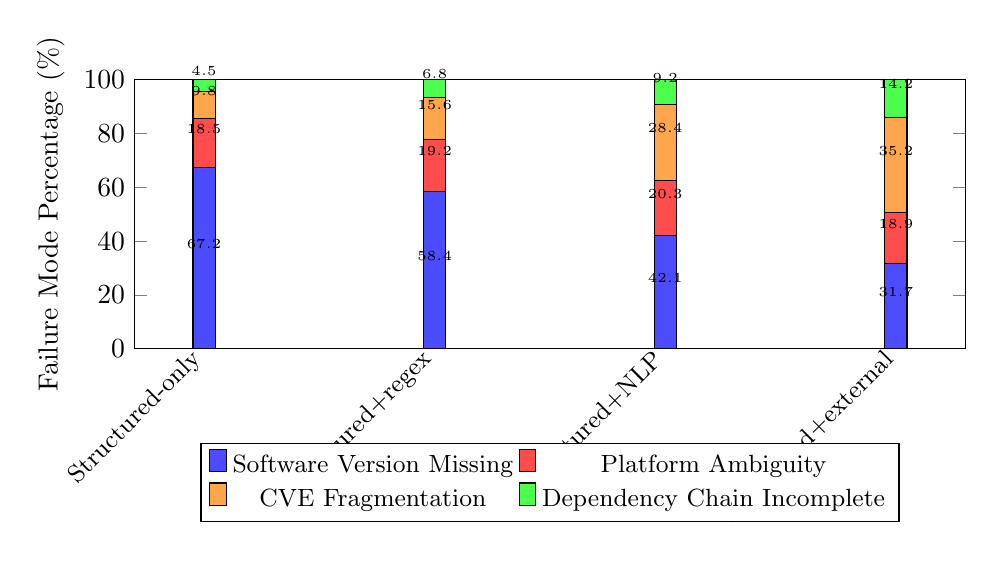
\begin{tikzpicture}
    \begin{axis}[
        ybar stacked,
        width=\textwidth,
        height=5cm,
        ylabel={Failure Mode Percentage (\%)},
        symbolic x coords={Structured-only, Structured+regex, Structured+NLP, Structured+external},
        xtick=data,
        x tick label style={rotate=45, anchor=east, font=\small},
        legend style={at={(0.5,-0.35)}, anchor=north, legend columns=2, font=\small},
        ymin=0, ymax=100,
        bar width=8pt,
        nodes near coords,
        nodes near coords align={vertical},
        every node near coord/.append style={font=\tiny},
    ]
    
    % Software version missing (dominant)
    \addplot[fill=blue!70] coordinates {
        (Structured-only, 67.2)
        (Structured+regex, 58.4)
        (Structured+NLP, 42.1)
        (Structured+external, 31.7)
    };
    
    % Platform ambiguity
    \addplot[fill=red!70] coordinates {
        (Structured-only, 18.5)
        (Structured+regex, 19.2)
        (Structured+NLP, 20.3)
        (Structured+external, 18.9)
    };
    
    % CVE fragmentation
    \addplot[fill=orange!70] coordinates {
        (Structured-only, 9.8)
        (Structured+regex, 15.6)
        (Structured+NLP, 28.4)
        (Structured+external, 35.2)
    };
    
    % Dependency chain incomplete
    \addplot[fill=green!70] coordinates {
        (Structured-only, 4.5)
        (Structured+regex, 6.8)
        (Structured+NLP, 9.2)
        (Structured+external, 14.2)
    };
    
    \legend{Software Version Missing, Platform Ambiguity, CVE Fragmentation, Dependency Chain Incomplete}
    \end{axis}
\end{tikzpicture}
